% Kettle-Stoker — the sixth class. Stoker: every four seconds the largest pool
% you are holding is shovelled into the furnace and comes back as one stack of
% mana empowerment, so the figure is a firebox with three hoppers over it and
% one of them going down.
%
% **Three hoppers, and only the full one is feeding.** That is the whole of the
% class: it burns the *largest* pool, so what you give up is the standing bonus
% you had been holding, and the decision is which hopper to fill. The other two
% stand there with their chutes shut.
%
% Counting is the house tic: nine rivets on the door, and the pressure gauge
% reads a number rather than a mood.
%
% Written by filling in tikz_figure_prompt.md.
\documentclass[tikz,border=4pt]{standalone}
\usetikzlibrary{calc}
\newcommand{\Unit}{0.055cm}
\newcommand{\Edge}{2.4pt}
\newcommand{\Rivets}{9}
\newcommand{\Coals}{6}

\definecolor{iron}{HTML}{5A5E66}
\definecolor{irondark}{HTML}{31343A}
\definecolor{fire}{HTML}{E0742A}
\definecolor{firepale}{HTML}{F2C255}
\definecolor{brass}{HTML}{C8A24A}
\definecolor{coal}{HTML}{22201E}
\definecolor{ink}{HTML}{101018}

\begin{document}
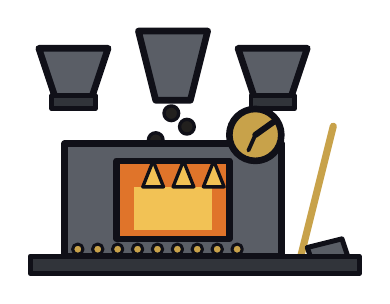
\begin{tikzpicture}[x=\Unit,y=\Unit, line join=round, line cap=round]

  % ---- three hoppers over the top -----------------------------------------
  % Left and right are shut. The middle one is the one going down, which is the
  % largest pool and is the thing you were holding.
  \fill[iron,draw=ink,line width=\Edge] (2,52) -- (18,52) -- (14,40) -- (6,40) -- cycle;
  \fill[iron,draw=ink,line width=\Edge] (48,52) -- (64,52) -- (60,40) -- (52,40) -- cycle;
  \fill[iron,draw=ink,line width=\Edge] (25,56) -- (41,56) -- (37,40) -- (29,40) -- cycle;
  % The shut chutes: a plate across the mouth of each.
  \fill[irondark,draw=ink,line width=1.8pt] (5,38) rectangle ++(10,3);
  \fill[irondark,draw=ink,line width=1.8pt] (51,38) rectangle ++(10,3);
  % And the open one, with coal coming out of it.
  \foreach \i in {1,...,\Coals} {
    \pgfmathsetmacro\x{29+mod(\i,3)*3.6}
    \pgfmathsetmacro\y{37-(\i-1)*3.1}
    \fill[coal,draw=ink,line width=1.2pt] (\x,\y) circle (1.7);
  }

  % ---- the furnace body ---------------------------------------------------
  \fill[iron,draw=ink,line width=\Edge] (8,4) rectangle (58,30);

  % ---- the door, open, and what is behind it ------------------------------
  \fill[fire,draw=ink,line width=\Edge] (20,8) rectangle (46,26);
  \fill[firepale] (24,10) rectangle (42,20);
  % The draught, drawn as three tongues rather than as a glow.
  \foreach \i in {0,1,2} {
    \pgfmathsetmacro\x{26+\i*7}
    \fill[firepale,draw=ink,line width=1.2pt]
      (\x,20) -- ({\x+2.4},26) -- ({\x+4.8},20) -- cycle;
  }

  % ---- nine rivets along the door frame -----------------------------------
  \foreach \i in {1,...,\Rivets} {
    \pgfmathsetmacro\x{11+(\i-1)*4.6}
    \fill[brass,draw=ink,line width=1.1pt] (\x,5.6) circle (1.2);
  }

  % ---- the gauge, which reads a number ------------------------------------
  \fill[brass,draw=ink,line width=\Edge] (52,32) circle (6);
  \draw[ink,line width=2.2pt] (52,32) -- ++(4.2,3.0);
  \draw[ink,line width=1.4pt] (52,32) -- ++(-1.6,-3.6);

  % ---- the shovel, leant against it ---------------------------------------
  \draw[brass,line width=2.6pt] (62,2) -- (70,34);
  \fill[iron,draw=ink,line width=1.8pt] (66,0) -- (74,2) -- (72,8) -- (64,6) -- cycle;

  % ---- the floor ----------------------------------------------------------
  \fill[irondark,draw=ink,line width=1.8pt] (0,0) rectangle (76,4);

\end{tikzpicture}
\end{document}
